\documentclass{article}
\usepackage[UTF8]{ctex}
\usepackage[tc]{titlepic}
\usepackage{titlesec}
\usepackage{cite}
\usepackage{fancyhdr}
\usepackage{booktabs}
\usepackage{graphicx}
\usepackage{geometry,float}
\usepackage[section]{placeins}
\geometry{a4paper,scale=0.8}
\pagestyle{fancy}

\lhead{第 1 次作业\\\today}
\chead{中国科学技术大学\\数学建模课程}

\rhead{Assignment 1\\ {\CTEXoptions[today=old]\today}}
\newcommand{\upcite}[1]{\textsuperscript{\cite{#1}}}

\titleformat*{\section}{\bfseries\Large}
\titleformat*{\subsection}{\bfseries\large}

\title{\bfseries 接缝裁剪}
\author{李奕萱 \quad  22 \quad  PB22000161}

\begin{document}
\maketitle
\begin{abstract}
    Seam Carving是一种创新的内容感知图像调整技术,
    通过智能地移除或添加最小能量的接缝来调整图像大小,
    同时最大限度地保留图像的重要内容。与传统的缩放方法
    相比,Seam Carving能够有效避免拉伸或压缩带来的失
    真,特别是在处理包含重要对象的图像时表现尤为出色。
    本文将详细探讨Seam Carving的原理、实现方法及其应用
    效果。
\end{abstract}
% \setcounter{secnumdepth}{1}
 \setcounter{section}{1}
\section*{\centerline{一、前言(问题的提出)}}
\subsection{传统图像缩放方法的局限性}
传统的图像缩放方法,如均匀采样和双线性插值,
虽然简单高效,但在调整大小时往往导致重要内容的失真。
例如,横向或纵向拉伸可能使人脸或物体变形,影响视觉效
果。此外,这些方法无法区分图像中重要区域和非重要区域,导致整体效果不理想。  \\
\subsection{Seam Carving简介}

Seam Carving通过计算图像中最小能量的接缝,选择性地
移除或添加这些接缝,从而在调整图像大小的同时,最大限
度地保留关键内容。这种方法在处理具有重要对象的图像时
尤其有效,能够避免传统方法的失真问题。
 \setcounter{section}{2}
\section*{\centerline{二、相关工作}}
Seam Carving技术由Avidor et al.首次提出\upcite{Avidan2007},
其核心思想在于通过计算图像的能量函数来确定最小能量的接缝。
随后的研究进一步优化了能量函数的计算方法和接缝的查找算法,
提升了Seam Carving的效率和效果。例如,研究者提出了多种改
进的能量函数,如对比度能量和梯度能量, 以更好地反映图像中
重要区域的分布。

接缝有两种形式,水平或垂直的。接缝本身是一条由像素构成的路径,
水平的接缝连接图像的左侧和右侧,路径中的像素个数和图像的列数一
致。垂直接缝则类似,连接图像的顶部和底部,像素个数和图像的行数
一致。接缝上每个像素都有存在一个称为重要性或者能量的指标,这个
指标的值是根据像素的邻接像素计算得到的。一个像素和周边像素的相
似度越高,则其重要性或者说能量就越低。

 \setcounter{section}{3}
\section*{\centerline{三、问题分析}}
    \subsection{能量函数的计算}
    能量函数是Seam Carving的核心,用于衡量图像中每个像素的重要性。
    常用的能量函数包括梯度能量和对比度能量。计算能量函数的准确性直
    接影响接缝的选择和最终的调整效果。然而,现有的能量函数可能无法
    完全反映图像中所有重要内容,例如复杂纹理或细微结构。
    \subsection{最小能量接缝的查找}
    在计算了能量函数后,需要在图像中找到具有最小累积能量的接缝。
    这一步涉及动态规划,以确保接缝的连贯性和最小能量的选择。
    然而,接缝的查找过程可能较为耗时,尤其是在处理高分辨率图像时。
    \subsection{多次调整的稳定性}
    在多次调整图像大小时,移除或添加接缝可能导致图像质量的逐步下降。
    因此,需要设计有效的策略来维持图像的稳定性和视觉一致性。例如,
    可以通过限制调整的次数或优化接缝的选择策略来减少图像质量的下降。
 \setcounter{section}{4}
\section*{\centerline{四、建模的假设}}
    \subsection{假设1:能量函数的合理性}
    假设图像中重要性较高的区域能量值较大,因此移除或添加低能量的
    接缝不会显著影响图像内容。这种假设在大多数情况下是合理的,但
    在某些特殊情况下(如图像中存在重要的低能量区域),可能会导致
    不理想的调整效果。
    \subsection{假设2:接缝的连贯性}
    假设移除或添加的接缝在水平或垂直方向上连贯,不会导致图像的破
    裂或明显的视觉不连续。这种假设确保了调整后的图像具有良好的视
    觉一致性,但在某些复杂场景中,可能需要进一步优化接缝的选择策
    略。
 \setcounter{section}{5}
 \section*{\centerline{五、符号说明}}
 \begin{table}[thb]
    \caption{\textbf{符号说明}}%标题
    \centering%把表居中
    \begin{tabular}{ccc}%内容全部居中
    \toprule%第一道横线
    符号&说明&单位 \\
    \midrule%第二道横线 
    $Im$ &输入图像 & - \\
    $E$ & 能量函数 & - \\
    $S$ & 最小能量接缝 & - \\
    $C$ & 累积能量矩阵 & - \\
    \bottomrule%第三道横线
    \end{tabular}
\end{table}

 \setcounter{section}{6}
\section*{\centerline{六、数学模型建立}}
Seam Carving的数学模型主要包括以下几个步骤:
\begin{enumerate}
    \item 计算能量函数:对于图像$Im$中的每个像素$(p, q)$,计
    算其能量值$E(p, q)$,通常使用梯度的大小表示: $ E(p, q) 
    = \sqrt{\left(\frac{\partial I}{\partial x}\right)
    ^2 + \left(\frac{\partial I}{\partial y}\right)^2} $、
    该公式通过计算图像的水平和垂直方向梯度的平方和的平方根,得到
    每个像素的能量值。能量值越高,表示该像素越重要。
    \item 构建累积能量矩阵:从图像的底部开始,向上计算每个像素
    的累积能量,确保接缝的连贯性: $ C(p, q) = E(p, q) + \min
    \left\{{C(p+1, q-1), C(p+1, q), C(p+1, q+1)}\right\} $
    该公式通过动态规划的方法,确保每个像素的累积能量是其自身能量
    值与上一行相邻像素中能量值最小的累积值之和。
    \item 查找最小能量接缝:从图像的顶部到底部,沿着累积能量最小
    的路径选择接缝: $ S = \arg\min\limits_{S} \sum\limits_{(p, q) \in S} 
    E(p, q) $
    通过回溯路径,找到具有最小累积能量的接缝路径。
    \item 移除或添加接缝:根据调整的需要,移除或添加选定的接缝,
    重构图像。移除接缝后,图像的尺寸会相应减小;添加接缝则可以实
    现图像的放大。
\end{enumerate}

 \setcounter{section}{7}
\section*{\centerline{七、结果(与对比)}}
    \subsection{结果展示}
    以下是Seam Carving算法在调整图像大小后的效果示例:
    \begin{figure}[htp]
        \centering %居中
        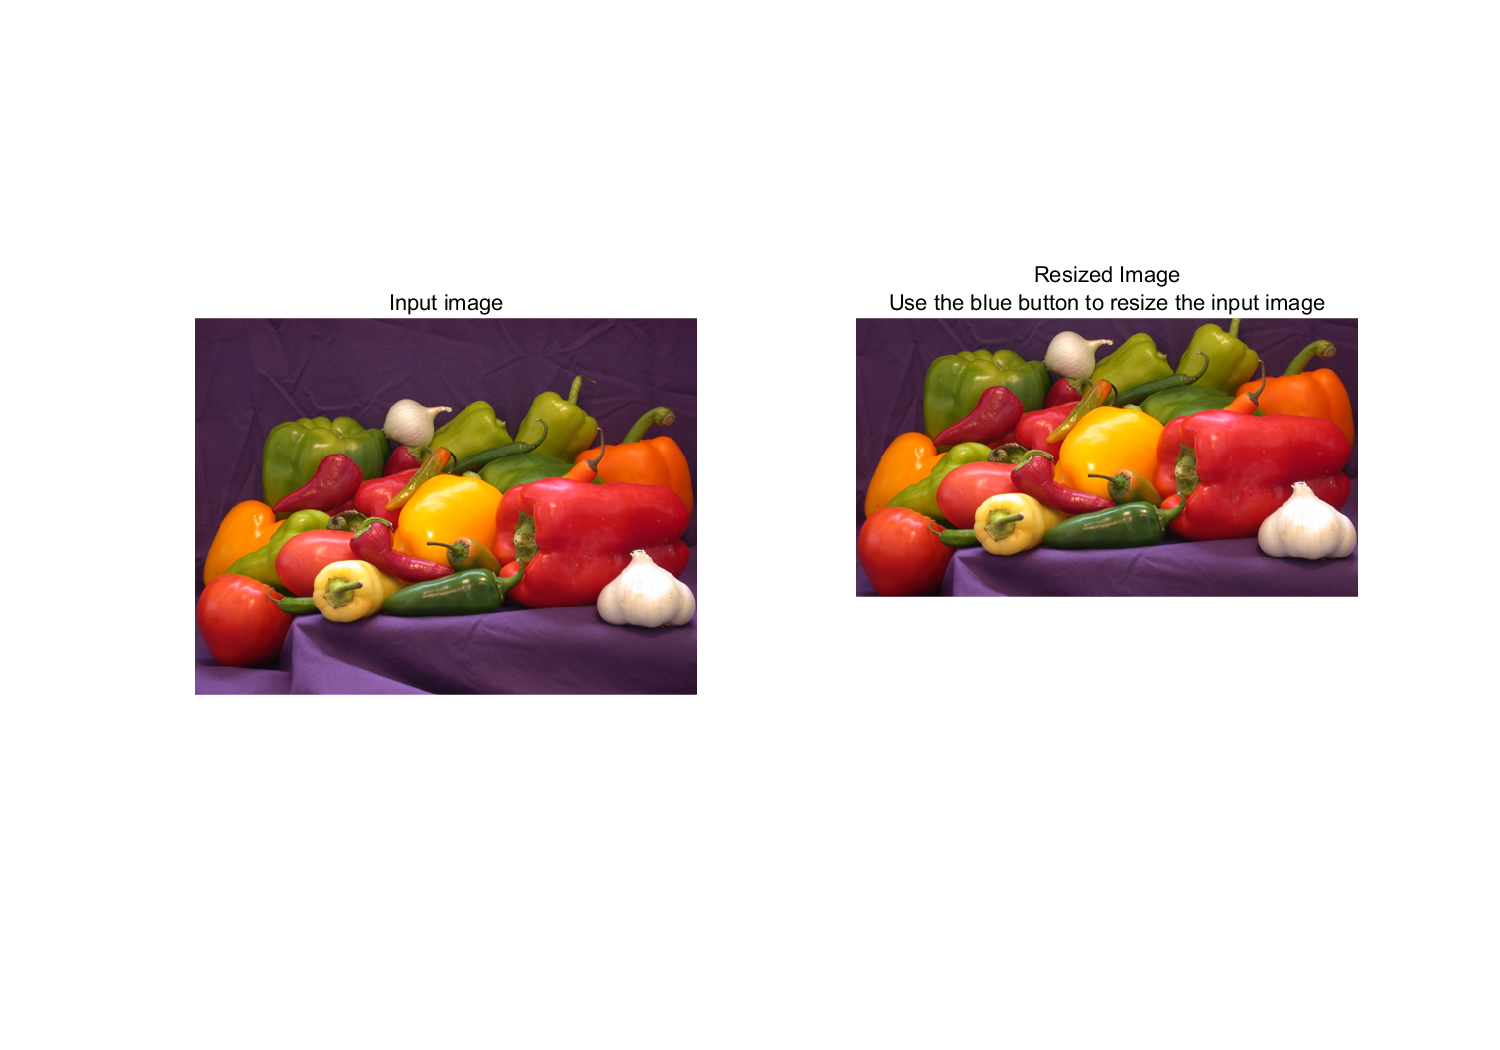
\includegraphics[width=0.7\textwidth]{jg2.png}
        \caption{高度减小100像素后的结果}
    \end{figure}
    \begin{figure}[htp]
        \centering %居中
        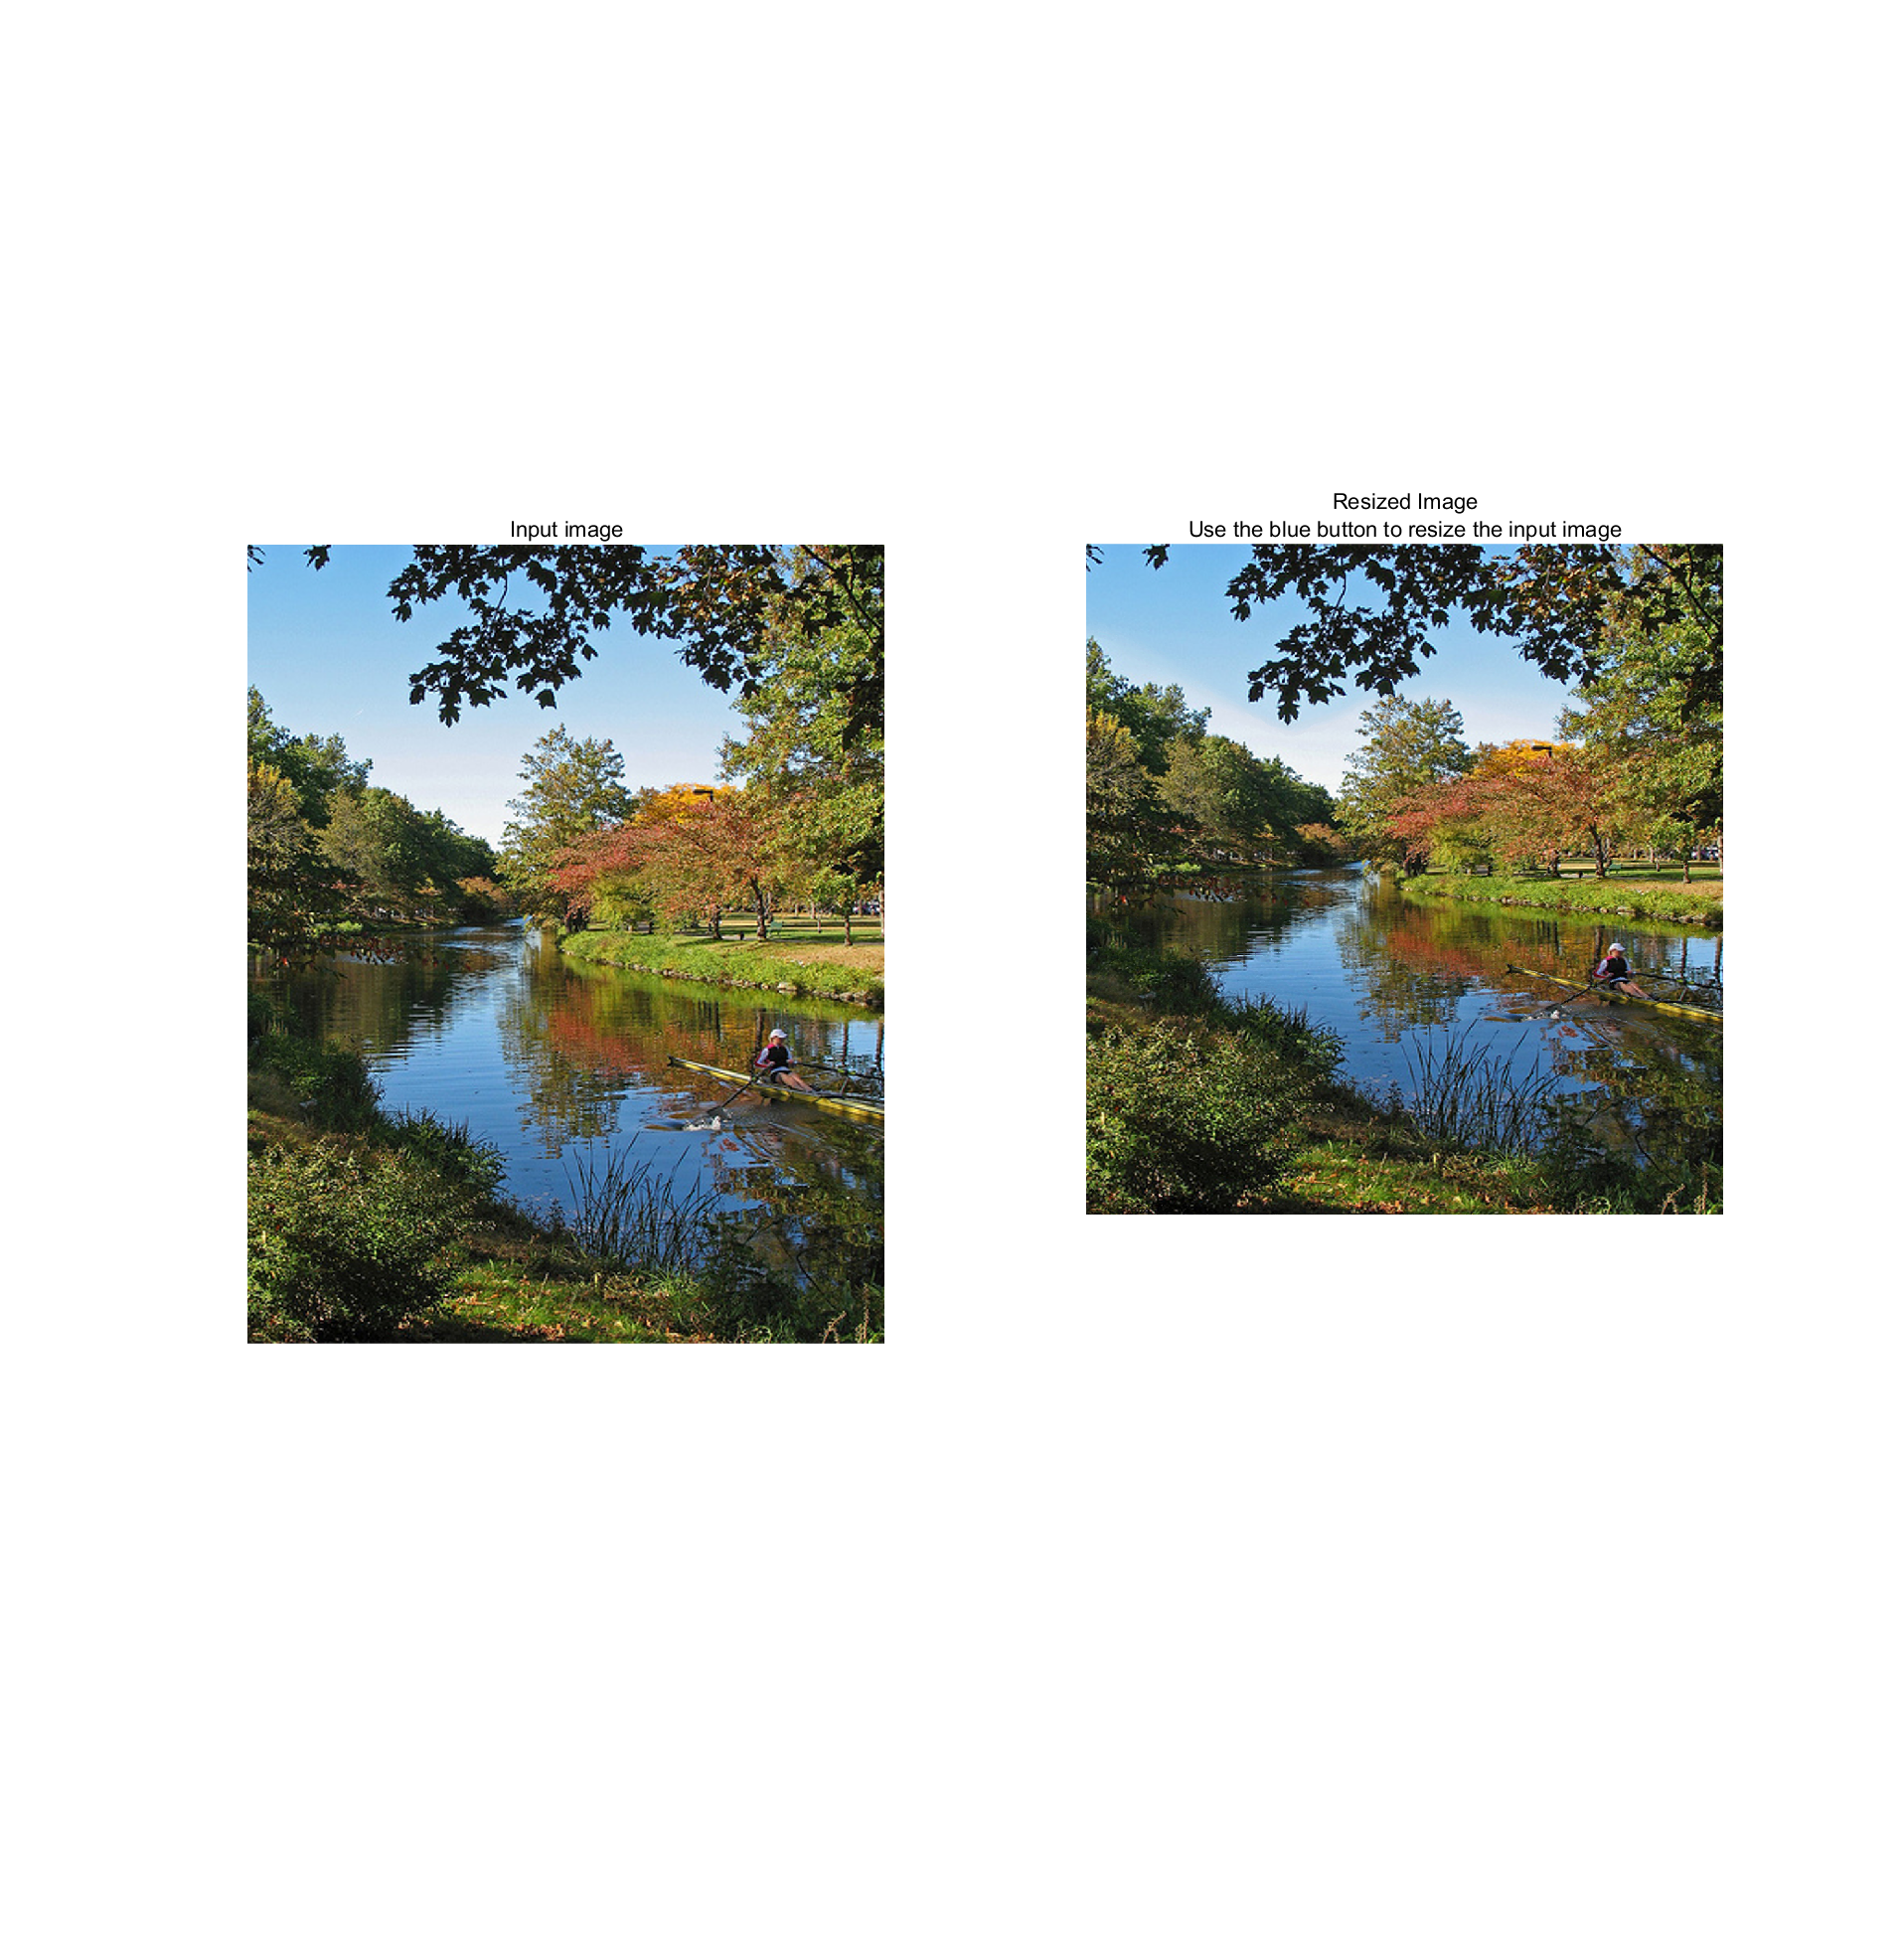
\includegraphics[width=0.7\textwidth]{jg1.png}
        \caption{高度减小200像素后的结果}
    \end{figure}
    \begin{figure}
    \centering %居中
    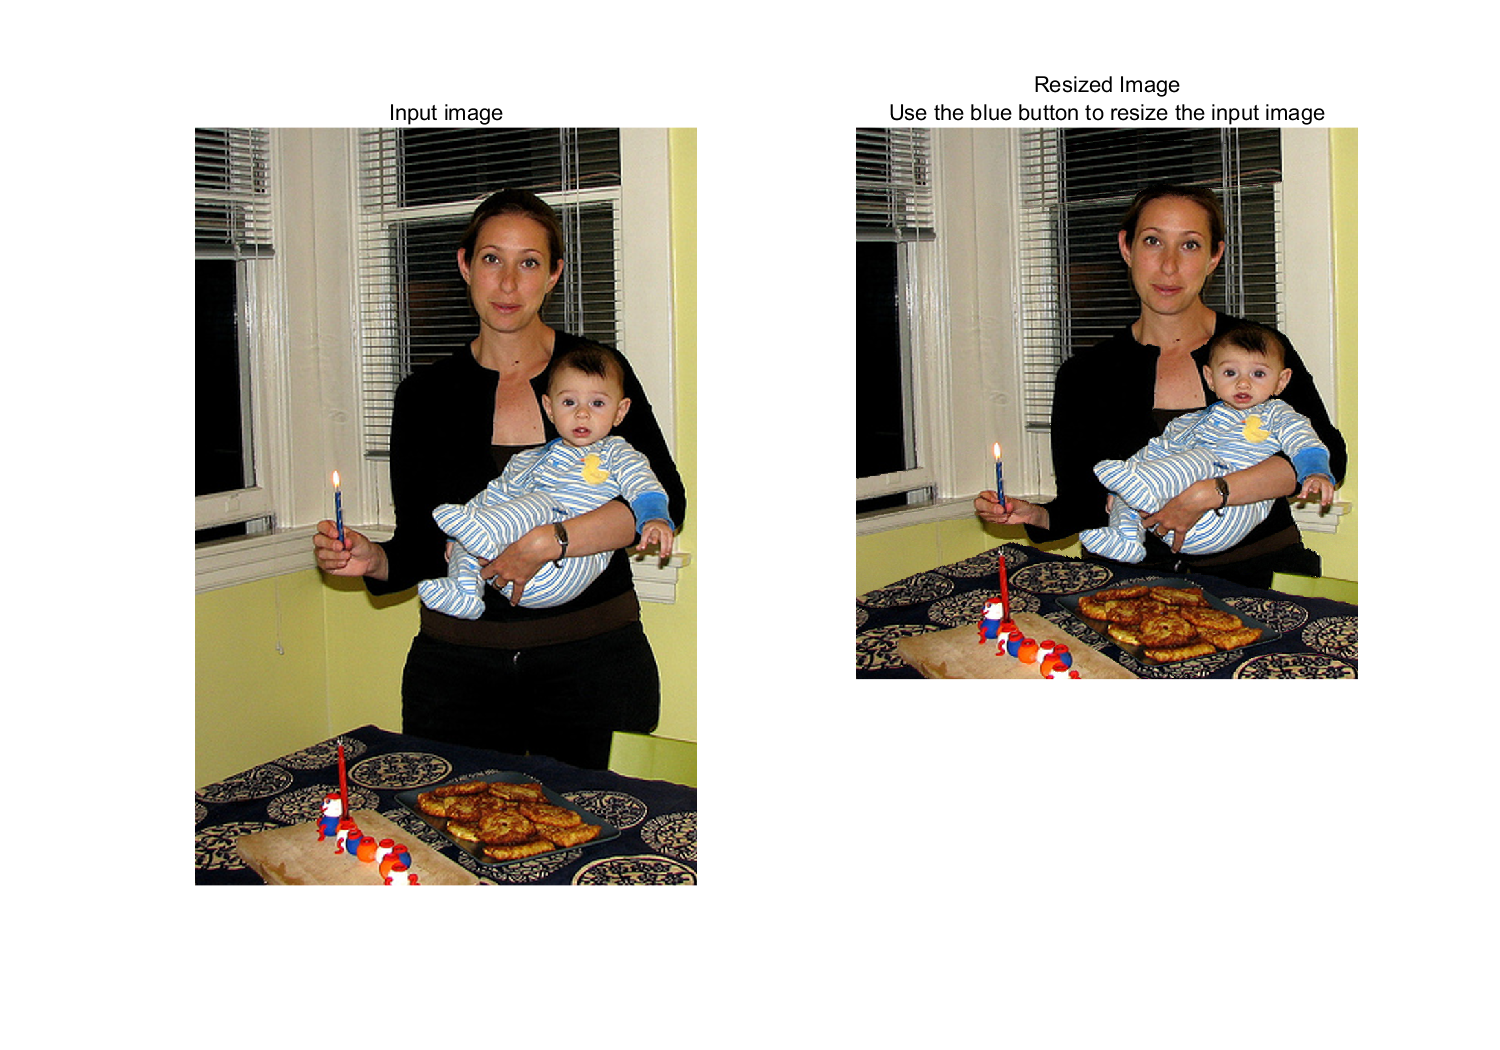
\includegraphics[width=0.8\textwidth]{jg6.png}
    \caption{高度减小300像素后的结果}
    \end{figure}
    \begin{figure}[htp]
        \centering %居中
        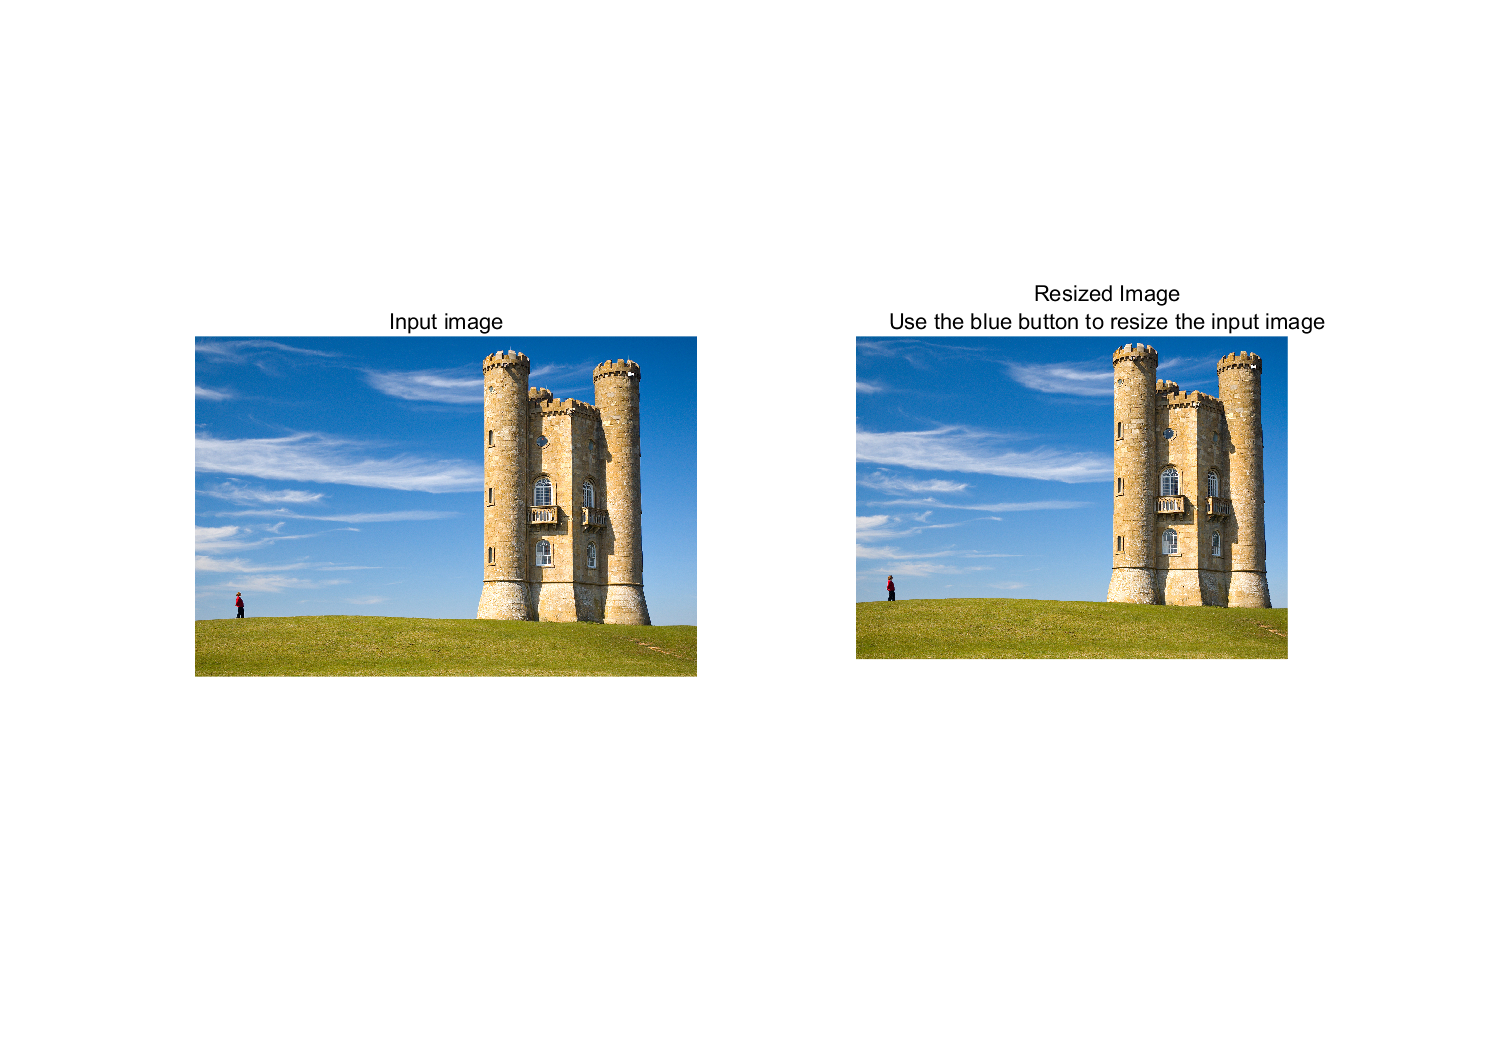
\includegraphics[width=0.8\textwidth]{jg4.png}
        \caption{宽度减小200,高度减小50像素后的结果}
    \end{figure}
    \begin{figure}[htp]
    \centering %居中
    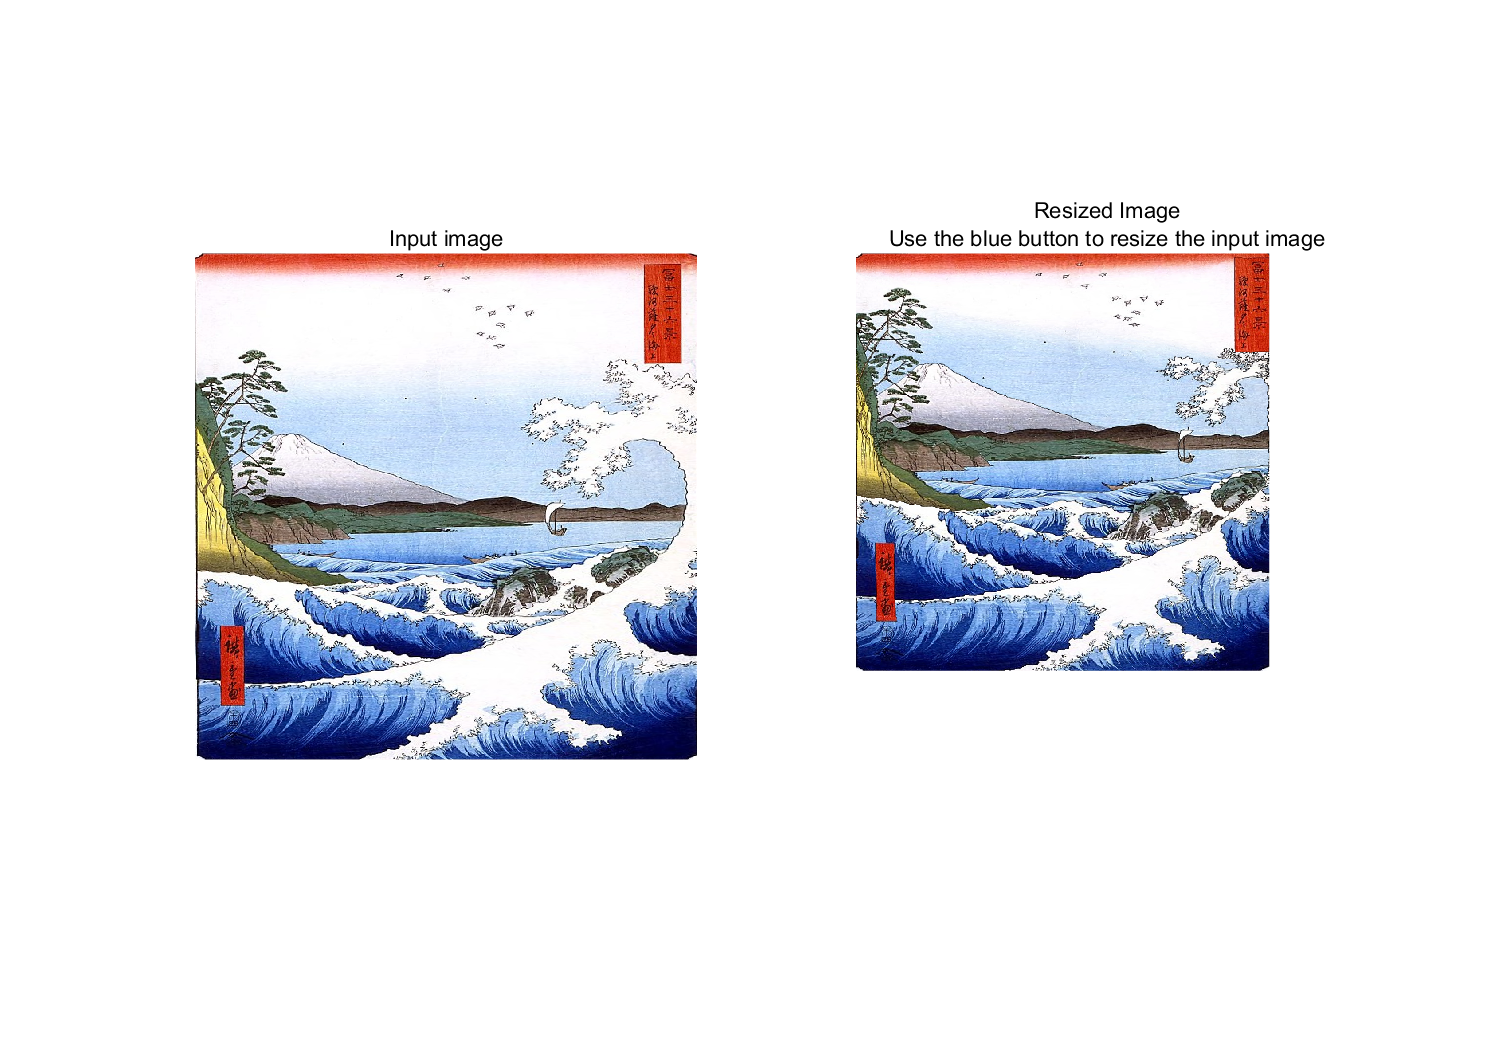
\includegraphics[width=0.8\textwidth]{jg5.png}
    \caption{宽度减小200,高度减小200像素后的结果}
    \end{figure}
    \begin{figure}[htp]
        \centering %居中
        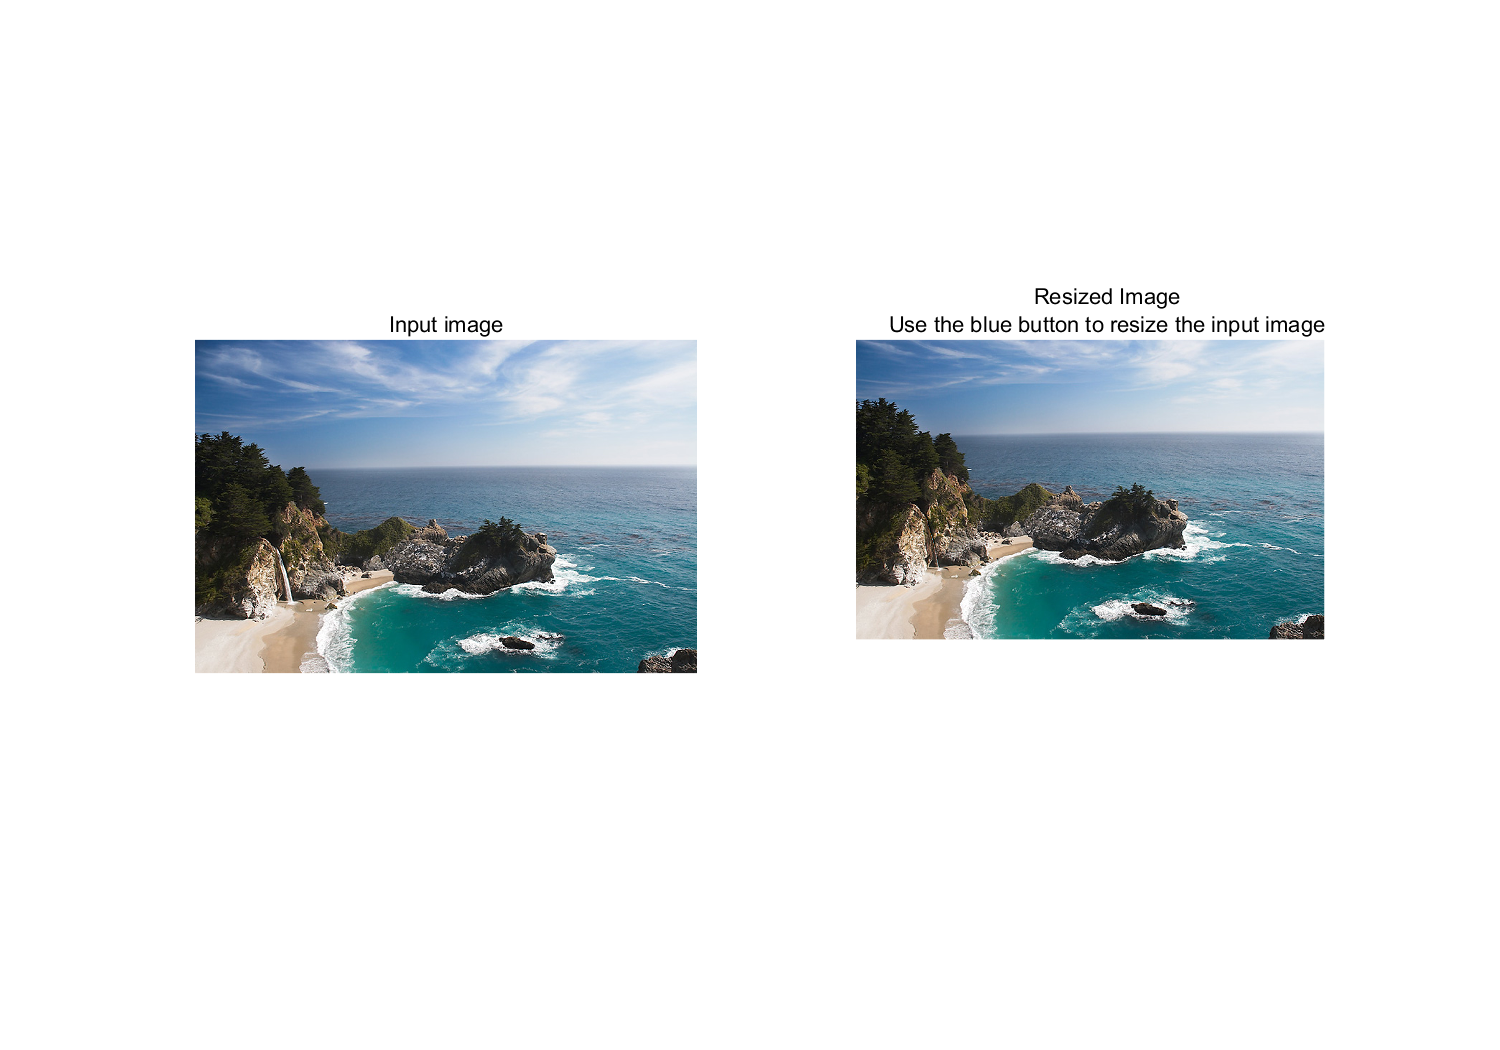
\includegraphics[width=0.8\textwidth]{jg3.png}
        \caption{宽度减小100,高度减小100像素后的结果}
    \end{figure}
    \subsection{结果对比}
    与传统的均匀采样方法相比,Seam Carving在调整后的图像中保留了
    更多的细节和重要内容,特别是在处理人脸和复杂纹理时表现尤为突出。
    例如,在缩小图像时,Seam Carving能够有效保护人脸的完整性,而
    均匀采样方法可能导致人脸变形。
 \setcounter{section}{8}
\section*{\centerline{八、结论}}
实验结果表明,Seam Carving在内容感知图像调整中具有显著优势,
能够有效避免传统方法的失真问题。其核心在于通过能量函数和最小接
缝的选择,实现了对重要内容的智能保护。 Seam Carving的应用前景广阔,
特别是在需要高质量图像调整的场景中。

 \setcounter{section}{9}
\section*{\centerline{九、问题}}
在实现Seam Carving过程中,仍存在一些问题和改进空间:

\begin{enumerate}
\item 计算效率:对于高分辨率图像,能量函数的计算和接
缝的查找可能较为耗时,需要优化算法以提升效率。
\item 能量函数的准确性:当前的能量函数可能无法完全反
映图像中所有重要内容,需要进一步研究更复杂的能量函数设计。
\item 多次调整的稳定性:在多次调整图像大小后,图像质
量可能逐渐下降,需要设计更稳定的调整策略。   
\end{enumerate}

\bibliographystyle{ieeetr}
\bibliography{refer}

\end{document}